\documentclass[12pt]{exam}
\usepackage{amsthm}
\usepackage{libertine}
\usepackage[utf8]{inputenc}
\usepackage[margin=1in]{geometry}
\usepackage{amsmath,amssymb}
\usepackage{multicol}
\usepackage[shortlabels]{enumitem}
\usepackage{siunitx}
\usepackage{booktabs}
\usepackage{graphicx}
\usepackage{pgfplots}
\usepackage{listings}
\usepackage{tikz}



\pgfplotsset{width=10cm,compat=1.9}
\usepgfplotslibrary{external}
%\tikzexternalize

\newcommand{\class}{Math 101-002} % This is the name of the course 
\newcommand{\examnum}{Exam 3} % This is the name of the assignment
\newcommand{\examdate}{April 17} % This is the due date





\begin{document}
\pagestyle{plain}
\thispagestyle{empty}

\noindent
\textbf{\class}\\
\textbf{\examnum}, \textbf{\examdate} \\

% Name \hfill CSU ID \# \hspace{2.25in}

%\vspace{10 pt}

\setlength{\tabcolsep}{3.5cm} % Default value: 6pt
\renewcommand{\arraystretch}{1.5}
\setlength\extrarowheight{1cm}
\begin{tabular}{ |c|c| } 
 \hline
 Name   & CSU ID \#  \\ 
 \hline
\end{tabular}
% ---
\vspace{10pt}

Be sure to read each question fully and carefully. Multiple choice answer bubbles must be fully filled in.  There is space to the right of each multiple choice question to show work, if your work is correct you can get points even with an incorrect multiple choice answer.  


\iffalse

    \foreach \s in {1,...,5}{
          \choice $P_\s$ has no power 
     }%;
\fi


\begin{enumerate} 

\item For questions \ref{firstQnSec1} through \ref{lastQnSec1} consider the following information about an electrical circuit:\par
\begin{figure}[h!]
    \centering
    \begin{tabular}{rrrr}\toprule
        Partition & Cycle type & Elements of conjugacy class\\ \midrule
        $(1,1,1,1)$& 4 1-cycles & $()$ (identity element)\\
        $(2,1,1)$& 1 transposition & $(12),(13),(14),$\\
        &&$(23),(24),(34)$\\
        $(2,2)$ & 2 transpositions & $(12)(34),(13)(24),(14)(23)$\\
        $(3,1)$ & 1 3-cycle& $(123),(132),(234),(243),$\\
        &&$(341),(314),(412),(421)$\\
        $(4)$ & 1 4-cycle & $(1234),(1243),(1324),$\\
        &&$(1342),(1423),(1432)$\\
   \bottomrule
    \end{tabular}
    \end{figure}

\begin{enumerate}
    \item \label{firstQnSec1} Based on the information presented in the tableux, fill in the edges of the graph $G$ representing this network: (4 points)
    \begin{figure}[h!]
        \centering
       
    
    
        \tikzset{every picture/.style={line width=0.75pt}} %set default line width to 0.75pt        
    
        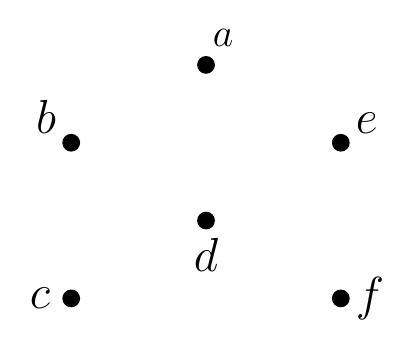
\begin{tikzpicture}[x=0.75pt,y=0.75pt,yscale=-1,xscale=1]
        %uncomment if require: \path (0,300); %set diagram left start at 0, and has height of 300
        
        %Shape: Circle [id:dp24175619248880365] 
        \draw  [fill={rgb, 255:red, 0; green, 0; blue, 0 }  ,fill opacity=1 ] (33.5,99.95) .. controls (33.5,97.74) and (35.29,95.95) .. (37.5,95.95) .. controls (39.71,95.95) and (41.5,97.74) .. (41.5,99.95) .. controls (41.5,102.16) and (39.71,103.95) .. (37.5,103.95) .. controls (35.29,103.95) and (33.5,102.16) .. (33.5,99.95) -- cycle ;
        %Shape: Circle [id:dp38562246159096747] 
        \draw  [fill={rgb, 255:red, 0; green, 0; blue, 0 }  ,fill opacity=1 ] (98.45,62.45) .. controls (98.45,60.24) and (100.24,58.45) .. (102.45,58.45) .. controls (104.66,58.45) and (106.45,60.24) .. (106.45,62.45) .. controls (106.45,64.66) and (104.66,66.45) .. (102.45,66.45) .. controls (100.24,66.45) and (98.45,64.66) .. (98.45,62.45) -- cycle ;
        %Shape: Circle [id:dp9956752087587961] 
        \draw  [fill={rgb, 255:red, 0; green, 0; blue, 0 }  ,fill opacity=1 ] (163.4,174.95) .. controls (163.4,172.74) and (165.19,170.95) .. (167.4,170.95) .. controls (169.61,170.95) and (171.4,172.74) .. (171.4,174.95) .. controls (171.4,177.16) and (169.61,178.95) .. (167.4,178.95) .. controls (165.19,178.95) and (163.4,177.16) .. (163.4,174.95) -- cycle ;
        %Shape: Circle [id:dp24033698556569782] 
        \draw  [fill={rgb, 255:red, 0; green, 0; blue, 0 }  ,fill opacity=1 ] (33.5,174.95) .. controls (33.5,172.74) and (35.29,170.95) .. (37.5,170.95) .. controls (39.71,170.95) and (41.5,172.74) .. (41.5,174.95) .. controls (41.5,177.16) and (39.71,178.95) .. (37.5,178.95) .. controls (35.29,178.95) and (33.5,177.16) .. (33.5,174.95) -- cycle ;
        %Shape: Circle [id:dp10560264310320788] 
        \draw  [fill={rgb, 255:red, 0; green, 0; blue, 0 }  ,fill opacity=1 ] (98.45,137.45) .. controls (98.45,135.24) and (100.24,133.45) .. (102.45,133.45) .. controls (104.66,133.45) and (106.45,135.24) .. (106.45,137.45) .. controls (106.45,139.66) and (104.66,141.45) .. (102.45,141.45) .. controls (100.24,141.45) and (98.45,139.66) .. (98.45,137.45) -- cycle ;
        %Shape: Circle [id:dp03400871765845248] 
        \draw  [fill={rgb, 255:red, 0; green, 0; blue, 0 }  ,fill opacity=1 ] (163.4,99.95) .. controls (163.4,97.74) and (165.19,95.95) .. (167.4,95.95) .. controls (169.61,95.95) and (171.4,97.74) .. (171.4,99.95) .. controls (171.4,102.16) and (169.61,103.95) .. (167.4,103.95) .. controls (165.19,103.95) and (163.4,102.16) .. (163.4,99.95) -- cycle ;
        
        % Text Node
        \draw (104.45,55.05) node [anchor=south west] [inner sep=0.75pt]  [font=\Large]  {$a$};
        % Text Node
        \draw (31.5,96.55) node [anchor=south east] [inner sep=0.75pt]  [font=\LARGE]  {$b$};
        % Text Node
        \draw (28.5,174.95) node [anchor=east] [inner sep=0.75pt]  [font=\LARGE]  {$c$};
        % Text Node
        \draw (102.45,144.85) node [anchor=north] [inner sep=0.75pt]  [font=\LARGE]  {$d$};
        % Text Node
        \draw (173.4,174.95) node [anchor=west] [inner sep=0.75pt]  [font=\LARGE]  {$f$};
        % Text Node
        \draw (173.4,96.55) node [anchor=south west] [inner sep=0.75pt]  [font=\LARGE]  {$e$};
        
        
        \end{tikzpicture}
    \end{figure}
    \vfill
    \item How many degrees of separation are there between $X$ and $Y$: (2 points)
    $$\deg(d)=\underline{\phantom{ans}}\quad\text{and}\quad\deg(e)=\underline{\phantom{ans}}.$$
    \vfill
    \item Write down two vertices of the graph with $7$ degrees of separation. (2 points)
    $$\deg(d)=\underline{\phantom{ans}}\quad\text{and}\quad\deg(e)=\underline{\phantom{ans}}.$$
    \vfill
    \item Based on the last question, the diameter of this graph should be \emph{at least}: (2 points)
    \begin{checkboxes}
        \choice 3
        \choice 6
        \choice 7
        \choice 8
    \end{checkboxes}
    \vfill
    \item The diameter of the graph $G$ is: (2 points)
    \vspace{0.5em}
    $$\operatorname{diam}(G)=\underline{\phantom{ans}}.$$
    \vfill
    \item The redundancy of the graph $G$ is: (2 points)
    \vspace{0.5em}
    $$\operatorname{red}(G)=\underline{\phantom{ans}}.$$
    \vfill
    \item A spanning tree of $G$ is {\Huge AQUIII}: (2 points)
    \begin{checkboxes}
        \choice $ab,bc,cd$
        \choice $ag,gc,cd$
        \choice $ag,ge,ed$
        \choice $af,fe,ed$
    \end{checkboxes}
    \vfill

    \item Write down the weight of the previous path: (2 points)
    \vspace{0.5em}
    $$\text{weight}=\underline{\phantom{ans}}.$$
    \vfill
    \item Does this graph $G$ have cut-edges (bridges)? (2 points)
    \begin{checkboxes}
        \choice Yes.
        \choice No.
    \end{checkboxes}
    \vfill
    \item State whether this graph has an Euler walk. If it does, write it down, if not state why it doesn't. (2 points)
    \vspace{8em}
    \vfill
    \item State whether this graph has an Hamilton walk. If it does, write it down, if not state why it doesn't. (2 points)
    \vspace{8em}
    \vfill
    \newpage
    \item The graph $G$ doesn't have an Euler circuit, Eulerize it by adding edges: (2 points)
    \begin{figure}[h]
        \centering
        \tikzset{every picture/.style={line width=0.75pt}} %set default line width to 0.75pt        
    
        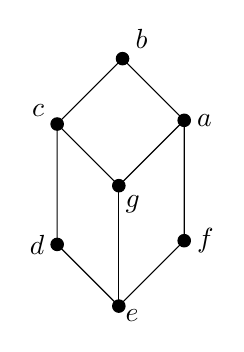
\begin{tikzpicture}[x=0.75pt,y=0.75pt,yscale=-1,xscale=1]
        %uncomment if require: \path (0,300); %set diagram left start at 0, and has height of 300
        
        %Shape: Cube [id:dp6646435130858394] 
        \draw   (30.79,59.04) -- (62.29,27.54) -- (92,57.25) -- (92,115.25) -- (60.5,146.75) -- (30.79,117.04) -- cycle ; \draw   (92,57.25) -- (60.5,88.75) -- (30.79,59.04) ; \draw   (60.5,88.75) -- (60.5,146.75) ;
        %Shape: Circle [id:dp7053935929182301] 
        \draw  [fill={rgb, 255:red, 0; green, 0; blue, 0 }  ,fill opacity=1 ] (59.29,27.54) .. controls (59.29,25.88) and (60.63,24.54) .. (62.29,24.54) .. controls (63.94,24.54) and (65.29,25.88) .. (65.29,27.54) .. controls (65.29,29.19) and (63.94,30.54) .. (62.29,30.54) .. controls (60.63,30.54) and (59.29,29.19) .. (59.29,27.54) -- cycle ;
        %Shape: Circle [id:dp3846430227043952] 
        \draw  [fill={rgb, 255:red, 0; green, 0; blue, 0 }  ,fill opacity=1 ] (89,57.25) .. controls (89,55.59) and (90.34,54.25) .. (92,54.25) .. controls (93.66,54.25) and (95,55.59) .. (95,57.25) .. controls (95,58.91) and (93.66,60.25) .. (92,60.25) .. controls (90.34,60.25) and (89,58.91) .. (89,57.25) -- cycle ;
        %Shape: Circle [id:dp3122259521210028] 
        \draw  [fill={rgb, 255:red, 0; green, 0; blue, 0 }  ,fill opacity=1 ] (57.5,88.75) .. controls (57.5,87.09) and (58.84,85.75) .. (60.5,85.75) .. controls (62.16,85.75) and (63.5,87.09) .. (63.5,88.75) .. controls (63.5,90.41) and (62.16,91.75) .. (60.5,91.75) .. controls (58.84,91.75) and (57.5,90.41) .. (57.5,88.75) -- cycle ;
        %Shape: Circle [id:dp5568900450079106] 
        \draw  [fill={rgb, 255:red, 0; green, 0; blue, 0 }  ,fill opacity=1 ] (27.79,59.04) .. controls (27.79,57.38) and (29.13,56.04) .. (30.79,56.04) .. controls (32.44,56.04) and (33.79,57.38) .. (33.79,59.04) .. controls (33.79,60.69) and (32.44,62.04) .. (30.79,62.04) .. controls (29.13,62.04) and (27.79,60.69) .. (27.79,59.04) -- cycle ;
        %Shape: Circle [id:dp5276475452889409] 
        \draw  [fill={rgb, 255:red, 0; green, 0; blue, 0 }  ,fill opacity=1 ] (27.79,117.04) .. controls (27.79,115.38) and (29.13,114.04) .. (30.79,114.04) .. controls (32.44,114.04) and (33.79,115.38) .. (33.79,117.04) .. controls (33.79,118.69) and (32.44,120.04) .. (30.79,120.04) .. controls (29.13,120.04) and (27.79,118.69) .. (27.79,117.04) -- cycle ;
        %Shape: Circle [id:dp01895932765963071] 
        \draw  [fill={rgb, 255:red, 0; green, 0; blue, 0 }  ,fill opacity=1 ] (57.5,146.75) .. controls (57.5,145.09) and (58.84,143.75) .. (60.5,143.75) .. controls (62.16,143.75) and (63.5,145.09) .. (63.5,146.75) .. controls (63.5,148.41) and (62.16,149.75) .. (60.5,149.75) .. controls (58.84,149.75) and (57.5,148.41) .. (57.5,146.75) -- cycle ;
        %Shape: Circle [id:dp8485087793178528] 
        \draw  [fill={rgb, 255:red, 0; green, 0; blue, 0 }  ,fill opacity=1 ] (89,115.25) .. controls (89,113.59) and (90.34,112.25) .. (92,112.25) .. controls (93.66,112.25) and (95,113.59) .. (95,115.25) .. controls (95,116.91) and (93.66,118.25) .. (92,118.25) .. controls (90.34,118.25) and (89,116.91) .. (89,115.25) -- cycle ;
        
        % Text Node
        \draw (97,57.25) node [anchor=west] [inner sep=0.75pt]    {$a$};
        % Text Node
        \draw (67.29,24.14) node [anchor=south west] [inner sep=0.75pt]    {$b$};
        % Text Node
        \draw (25.79,56.64) node [anchor=south east] [inner sep=0.75pt]    {$c$};
        % Text Node
        \draw (25.79,117.04) node [anchor=east] [inner sep=0.75pt]    {$d$};
        % Text Node
        \draw (62.5,147.15) node [anchor=north west][inner sep=0.75pt]    {$e$};
        % Text Node
        \draw (97,115.25) node [anchor=west] [inner sep=0.75pt]    {$f$};
        % Text Node
        \draw (62.5,92.15) node [anchor=north west][inner sep=0.75pt]    {$g$};
        
        
        \end{tikzpicture}
        
    \end{figure}
    \vfill 
    \item Assume you're traveling the graph $G$ and just came in to the $e$ from $d$. For $g$ to be your nearest neighbor, the weight of the edge $eg$ should be: (2 points)
    \begin{checkboxes}
        \choice 6
        \choice 12
        \choice 18
        \choice 24
    \end{checkboxes}
    \vfill
    \item When traveling the graph $G$, you arrived at the vertex $c$ from $b$. Following the Nearest-Neighbor algorithm, which vertex should you visit next? (2 points)
    \begin{checkboxes}
        \choice $a$
        \choice $b$
        \choice $d$
        \choice $g$
    \end{checkboxes}
    \vfill
    \item When applying the Cheapest-Link algorithm, suppose you have already picked the edges $ab$, $cd$, $ag$ and $cg$. Which edge should be picked next? (2 points)
    \begin{checkboxes}
        \choice $af$
        \choice $de$
        \choice $ef$
        \choice $bc$
    \end{checkboxes}
    \vfill
    \item \label{lastQnSec1} Suppose you're applying Cheapest-Link algorithm to $G$. For $eg$ to be $4^{\text{th}}$ edge you pick, its weight should be: (2 points)
    \vspace{0.5em}
    $$\text{weight}(eg)=\underline{\phantom{ans}}.$$
    \vfill
\end{enumerate}
\newpage
\item For questions \ref{firstQnSec2} through \ref{lastQnSec2} consider the information about the graph $G$ given by the following lists:
\begin{gather*}
    V=\left\lbrace a,b,c,d,e,f\right\rbrace,\\
    E=\left\lbrace ad,ae,bc,bd,cd,de,df,ea,ef\right\rbrace,\\
    W=\left\lbrace 7,10,4,6,5,9,8,6,7\right\rbrace.
\end{gather*}
The weights are ordered respecting the order of the edges.
\begin{enumerate}
\item \label{firstQnSec2} Fill in the weighted edges of the graph $G$ (Hint: Pay attention to the repeated edge): (4 points)
\begin{figure}[h!]
    \centering
   


    \tikzset{every picture/.style={line width=0.75pt}} %set default line width to 0.75pt        

    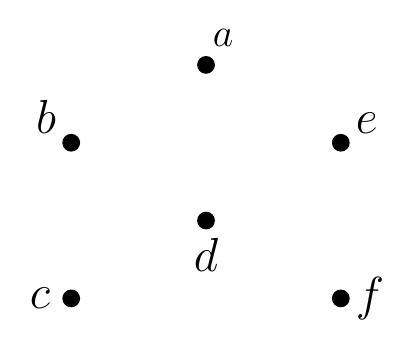
\begin{tikzpicture}[x=0.75pt,y=0.75pt,yscale=-1,xscale=1]
    %uncomment if require: \path (0,300); %set diagram left start at 0, and has height of 300
    
    %Shape: Circle [id:dp24175619248880365] 
    \draw  [fill={rgb, 255:red, 0; green, 0; blue, 0 }  ,fill opacity=1 ] (33.5,99.95) .. controls (33.5,97.74) and (35.29,95.95) .. (37.5,95.95) .. controls (39.71,95.95) and (41.5,97.74) .. (41.5,99.95) .. controls (41.5,102.16) and (39.71,103.95) .. (37.5,103.95) .. controls (35.29,103.95) and (33.5,102.16) .. (33.5,99.95) -- cycle ;
    %Shape: Circle [id:dp38562246159096747] 
    \draw  [fill={rgb, 255:red, 0; green, 0; blue, 0 }  ,fill opacity=1 ] (98.45,62.45) .. controls (98.45,60.24) and (100.24,58.45) .. (102.45,58.45) .. controls (104.66,58.45) and (106.45,60.24) .. (106.45,62.45) .. controls (106.45,64.66) and (104.66,66.45) .. (102.45,66.45) .. controls (100.24,66.45) and (98.45,64.66) .. (98.45,62.45) -- cycle ;
    %Shape: Circle [id:dp9956752087587961] 
    \draw  [fill={rgb, 255:red, 0; green, 0; blue, 0 }  ,fill opacity=1 ] (163.4,174.95) .. controls (163.4,172.74) and (165.19,170.95) .. (167.4,170.95) .. controls (169.61,170.95) and (171.4,172.74) .. (171.4,174.95) .. controls (171.4,177.16) and (169.61,178.95) .. (167.4,178.95) .. controls (165.19,178.95) and (163.4,177.16) .. (163.4,174.95) -- cycle ;
    %Shape: Circle [id:dp24033698556569782] 
    \draw  [fill={rgb, 255:red, 0; green, 0; blue, 0 }  ,fill opacity=1 ] (33.5,174.95) .. controls (33.5,172.74) and (35.29,170.95) .. (37.5,170.95) .. controls (39.71,170.95) and (41.5,172.74) .. (41.5,174.95) .. controls (41.5,177.16) and (39.71,178.95) .. (37.5,178.95) .. controls (35.29,178.95) and (33.5,177.16) .. (33.5,174.95) -- cycle ;
    %Shape: Circle [id:dp10560264310320788] 
    \draw  [fill={rgb, 255:red, 0; green, 0; blue, 0 }  ,fill opacity=1 ] (98.45,137.45) .. controls (98.45,135.24) and (100.24,133.45) .. (102.45,133.45) .. controls (104.66,133.45) and (106.45,135.24) .. (106.45,137.45) .. controls (106.45,139.66) and (104.66,141.45) .. (102.45,141.45) .. controls (100.24,141.45) and (98.45,139.66) .. (98.45,137.45) -- cycle ;
    %Shape: Circle [id:dp03400871765845248] 
    \draw  [fill={rgb, 255:red, 0; green, 0; blue, 0 }  ,fill opacity=1 ] (163.4,99.95) .. controls (163.4,97.74) and (165.19,95.95) .. (167.4,95.95) .. controls (169.61,95.95) and (171.4,97.74) .. (171.4,99.95) .. controls (171.4,102.16) and (169.61,103.95) .. (167.4,103.95) .. controls (165.19,103.95) and (163.4,102.16) .. (163.4,99.95) -- cycle ;
    
    % Text Node
    \draw (104.45,55.05) node [anchor=south west] [inner sep=0.75pt]  [font=\Large]  {$a$};
    % Text Node
    \draw (31.5,96.55) node [anchor=south east] [inner sep=0.75pt]  [font=\LARGE]  {$b$};
    % Text Node
    \draw (28.5,174.95) node [anchor=east] [inner sep=0.75pt]  [font=\LARGE]  {$c$};
    % Text Node
    \draw (102.45,144.85) node [anchor=north] [inner sep=0.75pt]  [font=\LARGE]  {$d$};
    % Text Node
    \draw (173.4,174.95) node [anchor=west] [inner sep=0.75pt]  [font=\LARGE]  {$f$};
    % Text Node
    \draw (173.4,96.55) node [anchor=south west] [inner sep=0.75pt]  [font=\LARGE]  {$e$};
    
    
    \end{tikzpicture}
\end{figure}
\vfill
\item List all the vertices adjacent to $d$: (2 points)
$$N(d)=\left\lbrace\underline{\phantom{ans}},\underline{\phantom{ans}},\underline{\phantom{ans}},\underline{\phantom{ans}},\underline{\phantom{ans}}\right\rbrace$$

\vfill
\item What are the degrees of the vertices $d$ and $e$? (4 points)
$$\deg(d)=\underline{\phantom{ans}}\quad\text{and}\quad\deg(e)=\underline{\phantom{ans}}.$$
\vfill
\item Find the sum of the degrees of all vertices: (2 points)
\begin{checkboxes}
    \choice 6
    \choice 9
    \choice 12
    \choice 18
\end{checkboxes}
\vfill
\item State whether this graph has an Euler walk. If it does, write it down, if not state why it doesn't. (2 points)
    \vspace{7em}
\vfill
\item The graph $G$ doesn't have an Euler circuit. Only one edge is needed to make it Eulerian. Which is that edge? (2 points)
  $$\text{missing edge}=\underline{\phantom{ans}}.$$
\vfill
\item Does this graph $G$ have cut-edges (bridges)? (2 points)
    \begin{checkboxes}
        \choice Yes.
        \choice No.
    \end{checkboxes}
    \vfill
\item What is the weight of the path $\left\lbrace bc,cd,df,fe\right\rbrace$? (2 points)
\begin{checkboxes}
    \choice 8
    \choice 16
    \choice 24
    \choice 28
\end{checkboxes}
\vfill
\item When traveling the graph $G$ starting at $e$, your Nearest-Neighbor algorithm took you to $a$ and then $d$. The next vertex you should visit is: (2 points)
\begin{checkboxes}
    \choice $b$
    \choice $c$
    \choice $e$
    \choice $f$
\end{checkboxes}
\vfill
\item The Nearest-Neighbor algorithm starting at the vertex $b$ produces a walk that ends at which vertex? (2 points)
\begin{checkboxes}
    \choice $a$
    \choice $b$
    \choice $d$
    \choice $f$
\end{checkboxes}
\vfill
\item \label{lastQnSec2} Which is the edge that you pick first in $G$ when applying the Cheapest-Link algorithm? (2 points)
$$1^{\text{st}}\text{edge}=\underline{\phantom{ans}}.$$
\vfill
\end{enumerate}
\newpage
\item Short answer:
\begin{enumerate}
    \item Explain the difference between a walk and a circuit of a graph. (4 points)
    \vspace{3cm}
    \item Explain the difference between Eulerian and Hamiltonian paths or circuits. (4 points)
    \vspace{3cm}
\end{enumerate}


\item In the following space draw the requested graphs:
\begin{enumerate}
    \item A graph with an Euler walk but without and Euler circuit. (4 points)
    \vspace{3.5cm}
    \item A graph with a Hamilton walk but without an Euler walk. (4 points)
    \vspace{3.5cm}
    \item A graph with an Euler circuit and a Hamilton walk, but not a Hamilton circuit. (4 points)
    \vfill
\end{enumerate}

\iffalse
Sol:
\begin{enumerate}
    \item A walk starts and ends at different places whereas a circuit begins and ends at the same place.
    \item Eulerian means that edges are the object of interest to traverse, while Hamiltonian means that the vertices are the traversed ones.
    \item Any path graph.
    \item A path graph with any pair of middle vertices connected.
    \item Two triangles joined at a vertex, say a ribbon.
    \item The ribbon graph again.
    \item A cycle with more than four vertices with any two non-adjacent vertices connected.
\end{enumerate}
\fi
\newpage
\item (25 points) Realistically, when you're traveling in your local city, you're very likely to know your neighborhood and your route to your worksite. It is also likely that you know the places you frequent often such as the supermarket and houses of friends you visit often.\par
In this hypothetical scenario, you're driving to a concert this weekend and need to pick up several friends along the way. Some friends live close to you, while others are farther away in areas you're not familiar with. You also don't know the concert venue very well.\par
For this scenario, assume you have a physical map of the city and the addresses of your friends, but no access to GPS or navigation apps.\par
In the following space address the following prompts and discuss thoroughly and explain your reasonings:
\begin{itemize}
    \item Do you think that this situation is better modeled through an Eulerian or Hamiltonian approach? Are you trying to make a walk or a circuit? 
    \item Since some friends live nearby and others farther away, where you're not familiar, would that influence your choice of algorithm to pick up? Why?
    \item Could a mix of algorithms make for a better route?
    \item If you're running late or some friends aren't ready yet, how does that change your approach? Would it affect your choice of algorithm or the order in which you pick people up? Why or why not?
\end{itemize}

Sol:
\begin{itemize}
    \item 8 pts clearly explains whether the situation is more Hamilton or Euler and adds evidence to support reasonings.
    \item 6 pts discusses how friends locations affects choice of approach
    \item 6 pts thoroughly considers whether a hybrid strategy would be beneficial.
    \item 5 pts similarly discusses how a time constraint could affect the choice.
\end{itemize}

\end{enumerate}
\end{document}

